\documentclass[12pt,a4paper,twoside]{book}
% Language setup for Greek and English
\usepackage[english,greek]{babel}
\usepackage[utf8]{inputenc}
\usepackage[T1,LGR]{fontenc}
% Font setup
\usepackage{fontspec}
\setmainfont{Linux Libertine O}[Scale=0.9]
\setsansfont{Linux Biolinum}[Scale=0.9]
\setmonofont{DejaVu Sans Mono}[Scale=0.9]
% Other necessary packages
\usepackage{enumitem}
\usepackage{graphicx}
\usepackage{amsmath}
\usepackage{makeidx}
\usepackage{multicol}
\usepackage{multirow}
\usepackage{hanging}
\usepackage{adjustbox}
\usepackage{amssymb}
\usepackage{stackengine}
\usepackage{ifthen}
\usepackage{array}
\usepackage{tcolorbox}
\tcbuselibrary{skins,breakable}
\usepackage{minted}
\usepackage{listings}
\usepackage{parskip}
\usepackage{float}
\usepackage{subcaption}
\usepackage{xcolor}
\usepackage{cancel}
\usepackage{pdfpages}
\usepackage{titlesec}
% Page & text layout
\usepackage{geometry}
\geometry{
   a4paper,
   top=2.5cm,
   bottom=2.5cm,
   left=2.5cm,
   right=2.5cm
}
% Headers & footers
\usepackage{fancyhdr}
\pagestyle{fancyplain}
\renewcommand{\footrulewidth}{0.4pt}
% Hyperlinks
\usepackage{hyperref}
\usepackage{bookmark} % Add this line to fix the hyperref warnings
\hypersetup{
    colorlinks=true,
    linkcolor=blue,
    citecolor=blue,
    filecolor=blue,
    urlcolor=cyan,
    unicode,
    pdftitle={3η Εργαστηριακή Άσκηση Τεχνητής Νοημοσύνης},
    pdfsubject={Τεκμηρίωση},
    pdfborderstyle={/S/U/W 1}, % Underline links
}
\usepackage{tikz}
\usetikzlibrary{positioning, shapes.geometric, arrows.meta}

% Define Command Line settings for listings
\lstdefinestyle{myCstyle}{
  language=C, % Set the language to C
  backgroundcolor=\color{white}, % Background color of the listing
  basicstyle=\ttfamily\footnotesize, % Basic font style and size
  keywordstyle=\color{blue}\bfseries, % Style for keywords
  commentstyle=\color{green!60!black}\itshape, % Style for comments
  stringstyle=\color{orange}, % Style for strings
  showstringspaces=false, % Don't show spaces in strings
  frame=single, % Frame around the code block
  rulecolor=\color{gray}, % Color of the frame
  breaklines=true, % Automatically break long lines
  numbers=left, % Line numbers on the left
  numberstyle=\tiny\color{gray}, % Style for line numbers
  tabsize=4, % Size of a tab
  captionpos=b, % Position of the caption (b for bottom)
  morekeywords={uint32_t, uint8_t, int, char, double, boolean, String, class, new, return, void, if, else, while, do, for, switch, case, default, break, true, false, public, private, var, string}, % Add additional keywords
  escapeinside={\(*@}{@*\)} % for escaping characters
}

\definecolor{customRed}{HTML}{FF5F5A} % using hexadecimal
\definecolor{customYellow}{HTML}{FFBE2E} % using hexadecimal
\definecolor{customGreen}{HTML}{2ACA44} % using hexadecimal
\definecolor{customPurple}{HTML}{C477DB} % using hexadecimal
\definecolor{customBlue}{HTML}{052538} % using hexadecima
\definecolor{customLightBlue}{HTML}{60ADEC} % using hexadecimall

\lstdefinestyle{myPythonStyle}{
    language=Python, % Set the language to Python
    backgroundcolor=\color{customBlue}, % Background color
    basicstyle=\color{customRed}\ttfamily\footnotesize, % Basic font style, size, and color
    keywordstyle=\color{customPurple}\bfseries, % Style for general keywords
    keywordstyle=[2]\color{customYellow}\bfseries, % Style for specific keywords
    morekeywords=[2]{os, graphviz, Digraph, collections, deque, math, tabulate}, % Define 'import' and 'from' as additional keywords
    commentstyle=\color{gray}\itshape, % Style for comments
    stringstyle=\color{customGreen}, % Style for strings
    identifierstyle=\color{customLightBlue}, % Style for identifiers
    % procnamekeys={def,class}, % Highlight function and class names
    showstringspaces=false, % Don't show spaces in strings
    frame=none, % No frame around the code block
    rulecolor=\color{black}, % Color of the frame (if enabled)
    breaklines=true, % Automatically break long lines
    numbers=left, % Line numbers on the left
    numberstyle=\small\color{gray}, % Style for line numbers
    % numwidth=4em, % Width allocated for line numbers
    stepnumber=1, % Step between line numbers
    numbersep=8pt, % Distance of line numbers from code
    xleftmargin=1em,           % Match the numwidth
    tabsize=4, % Size of a tab
    captionpos=t, % Position of the caption (t for top)
    firstnumber=auto, % Continue line numbering from previous listing
    aboveskip=0em,    % Remove external spacing
    belowskip=0em,    % Remove external spacing
    framesep=1em,     % Add internal padding
    %   framexleftmargin=1em, % Add internal left margin
    %   framexrightmargin=1em, % Add internal right margin
    frame=tb,         % Add top and bottom rules only
    framerule=0pt,    % Make the rules invisible
    morekeywords={self, None, True, False, format, abs, as, pass, return, if, elif, else, for, range, while, try, except, with, lambda, yield, global, nonlocal, assert, del, raise, in, is, and, or, not}, % Additional keywords
    escapeinside={\(*@}{@*\)}, % For escaping characters
    morecomment=[l]{\#}, % Define comment style
    morestring=[b]', % Define string style with single quotes
    morestring=[b]", % Define string style with double quotes % chktex 18
}

\tcbset{
  myCustomStyle/.style={
    enhanced,                    % Enable enhanced features
    colback=customBlue,         % Background color
    colframe=black!75,          % Frame color
    fonttitle=\bfseries,        % Title font style
    % frame=single,               % Frame type
    % interior titled,            % Use regular titled interior
    interior style={
      top color=black!75,       % Title area background
      bottom color=black!75,    % Title area background
    },
    colbacktitle=black!75,      % Title background color
    coltitle=white,             % Title color
    rounded corners,            % Rounded corners
    boxrule=1mm,               % Frame thickness
    drop shadow southeast,      % Shadow effect
    lefttitle=0pt,             % Remove left margin of title
    % left=1em,                  % Increase left margin for line numbers
    title={\hspace*{-1.25em}\textcolor{customRed}{● }\textcolor{customYellow}{● }\textcolor{customGreen}{●}\quad#1}, % Circles + Title
    attach title to upper={\vspace{2.3mm}}, % Adjust vertical spacing
    beforeafter skip=8pt,      % Space before and after the box
    % sharp corners              % Sharp corners for the title area
  }
}

% Custom commands for language switching
\newcommand{\en}[1]{\foreignlanguage{english}{#1}}
\newcommand{\gr}[1]{\foreignlanguage{greek}{#1}}
% Custom command for coloring
\newcommand{\blue}[1]{\textcolor{blue}{#1}}
% Index
\makeindex
% Set headheight to avoid fancyhdr warnings
\setlength{\headheight}{14.5pt}

\begin{document}

% Set main language to Greek
\selectlanguage{greek}

\begin{titlepage}
	\vspace*{8cm}
	\begin{center}
		{\LARGE \textbf{Νευρωνικά Δίκτυα - Perceptron}}\\ % chktex 8
		\vspace*{0.5cm}
		{\large 3η Εργαστηριακή Άσκηση}\\
		{\large Τεχνητή Νοημοσύνη}
		\vspace*{5cm}
		\\
		\vspace*{1cm}
		\begin{tabular}{l l l l}
			\large Βασίλειος Μπίτζας & \large 1083796 & \large 4o & \large
		\end{tabular}

		\vspace*{1cm}

		{\normalsize Τμήμα Μηχανικών Η/Υ \& Πληροφορικής}
		\\
		{\normalsize Πανεπιστήμιο Πατρών}
		\\
	\end{center}
	\thispagestyle{empty} % Suppress page number on the title page
\end{titlepage}

% Suppress page number on the subsequent page
\pagenumbering{gobble}
% Add this command to prevent blank pages
\let\cleardoublepage\clearpage
\frontmatter
\tableofcontents
\mainmatter % chktex 1

\chapter{Ανάλυση Υλοποίησης Perceptron}

\section{Εισαγωγή}
Η παρούσα υλοποίηση αφορά ένα απλό perceptron, το οποίο είναι ένα από τους βασικότερους τύπους τεχνητών νευρώνων. Το perceptron χρησιμοποιείται για δυαδική ταξινόμηση, διαχωρίζοντας τα δεδομένα σε δύο κλάσεις.

\section{Κλάση Perceptron}

\subsection{Δομή και Μεταβλητές}

\begin{tcolorbox}[myCustomStyle = {perceptron.py}]
    \begin{lstlisting}[style=myPythonStyle]
 class Perceptron:
     def __init__(self, learning_rate = 0.01, epochs = 100):
         self.learning_rate = learning_rate  # "Ρυθμός μάθησης"
         self.epochs = epochs                # "Αριθμός εποχών"
         self.weights = None                 # Βάρη
         self.bias = 0                       # Μεροληψία
         self.errors = []                    # "Καταγραφή σφαλμάτων"
    \end{lstlisting}
\end{tcolorbox}

Η κλάση Perceptron περιλαμβάνει τις εξής βασικές μεταβλητές:
\begin{itemize}
    \item \textbf{\texttt{learning\_rate}}: Καθορίζει το μέγεθος του βήματος προσαρμογής των βαρών
    \item \textbf{\texttt{epochs}}: Ορίζει τον αριθμό επαναλήψεων της εκπαίδευσης
    \item \textbf{\texttt{weights}}: Αποθηκεύει τα βάρη του perceptron
    \item \textbf{\texttt{bias}}: Αποθηκεύει τη μεροληψία του perceptron
    \item \textbf{\texttt{errors}}: Καταγράφει τα σφάλματα ανά εποχή
\end{itemize}

\subsection{Αναλυτική Λειτουργία της Μεθόδου Εκπαίδευσης (fit)}

\begin{tcolorbox}[myCustomStyle = {perceptron.py}]
    \begin{lstlisting}[style=myPythonStyle]
 def fit(self, X, y):
     n_features = len(X[0])
     self.weights = [0.0] * n_features
     self.bias = 0
    \end{lstlisting}
\end{tcolorbox}

Η μέθοδος \textbf{\textit{fit}()} λειτουργεί ως εξής: % chktex 36

\begin{enumerate}
    \item \textbf{Αρχικοποίηση}:
    \begin{itemize}
        \item Δημιουργεί διάνυσμα βαρών μηδενικών τιμών με μέγεθος ίσο με τον αριθμό χαρακτηριστικών
        \item Αρχικοποιεί τη μεροληψία (bias) στο μηδέν
    \end{itemize}
    \item \textbf{Διαδικασία Εκπαίδευσης}:
    \begin{itemize}
        \item Επαναλαμβάνει για κάθε εποχή:
        \begin{itemize}
            \item Υπολογίζει την έξοδο για κάθε δείγμα εκπαίδευσης
            \item Συγκρίνει την πρόβλεψη με την πραγματική τιμή
            \item Ενημερώνει τα βάρη και τη μεροληψία όταν υπάρχει σφάλμα
        \end{itemize}
    \end{itemize}
    \item \textbf{Ενημέρωση Βαρών}:
    Όταν η πρόβλεψη είναι λανθασμένη:
    \begin{tcolorbox}[myCustomStyle = {perceptron.py}]
        \begin{lstlisting}[style=myPythonStyle]
 update = self.learning_rate * y[i]
 self.weights = [w + update * x for w, x in zip(self.weights, X[i])]
 self.bias += update
        \end{lstlisting}
    \end{tcolorbox}
\end{enumerate}

\subsection{Λεπτομερής Περιγραφή της Μεθόδου Πρόβλεψης (predict)}

\begin{tcolorbox}[myCustomStyle = {perceptron.py}]
    \begin{lstlisting}[style=myPythonStyle]
 def predict(self, X):
    \end{lstlisting}
\end{tcolorbox}

Η μέθοδος \textbf{\textit{predict}()} εκτελεί: %chktex 36

\begin{enumerate}
    \item \textbf{Υπολογισμός Γραμμικής Εξόδου}:
    \begin{itemize}
        \item Πολλαπλασιάζει κάθε χαρακτηριστικό με το αντίστοιχο βάρος
        \item Προσθέτει τη μεροληψία
        \item Εφαρμόζει τη συνάρτηση ενεργοποίησης \textit{sign}() %chktex 36
    \end{itemize}
    \item \textbf{Επιστροφή Προβλέψεων}:
    \begin{itemize}
        \item Επιστρέφει λίστα με τις προβλέψεις (-1 ή +1)
    \end{itemize}
\end{enumerate}

\section{Βοηθητικές Συναρτήσεις}

\subsection{Συνάρτηση linspace}

\begin{tcolorbox}[myCustomStyle = {perceptron.py}]
    \begin{lstlisting}[style=myPythonStyle]
 def linspace(start, stop, num):
     """Αντικατάσταση της numpy linspace"""
     if num == 1:
         return [start]
     step = (stop - start) / (num - 1)
     return [start + i * step for i in range(num)]
    \end{lstlisting}
\end{tcolorbox}

Η συνάρτηση \textbf{linspace} υλοποιεί την αντίστοιχη λειτουργικότητα της \textbf{numpy.linspace}:
\begin{itemize}
    \item \textbf{Είσοδος}:
    \begin{itemize}
        \item \textbf{\texttt{start}}: Αρχική τιμή του διαστήματος
        \item \textbf{\texttt{stop}}: Τελική τιμή του διαστήματος
        \item \textbf{\texttt{num}}: Αριθμός σημείων
    \end{itemize}
    \item \textbf{Έξοδος}: Λίστα με \textbf{num} ισαπέχοντα σημεία
    \item \textbf{Χρήση}: Χρησιμοποιείται για τη δημιουργία σημείων στη γραφική απεικόνιση
\end{itemize}

\subsection{Συνάρτηση load\_data}

\begin{tcolorbox}[myCustomStyle = {perceptron.py}]
    \begin{lstlisting}[style=myPythonStyle]
 def load_data(filename):
     X, y = [], []
     with open(filename, 'r') as f:
         next(f)  # "Παράλειψη κεφαλίδας"
         for line in f:
             x1, x2, label = map(float, line.strip().split(','))
             X.append([x1, x2])
             y.append(1 if label == 1.0 else -1)
     return X, y
    \end{lstlisting}
\end{tcolorbox}

Η συνάρτηση \textbf{load\_data} διαχειρίζεται την ανάγνωση και επεξεργασία των δεδομένων:
\begin{itemize}
    \item \textbf{Λειτουργία}:
    \begin{itemize}
        \item Διαβάζει αρχείο CSV με δεδομένα εκπαίδευσης ή ελέγχου
        \item Παραλείπει την πρώτη γραμμή (κεφαλίδες)
        \item Μετατρέπει τις τιμές σε αριθμούς κινητής υποδιαστολής
        \item Διαχωρίζει τα χαρακτηριστικά (X) από τις ετικέτες (y)
    \end{itemize}
    \item \textbf{Επιστρεφόμενες τιμές}:
    \begin{itemize}
        \item \texttt{X}: Λίστα με ζεύγη τιμών [x₁, x₂]
        \item \texttt{y}: Λίστα με ετικέτες κλάσεων (+1 ή -1)
    \end{itemize}
\end{itemize}

\subsection{Συνάρτηση get\_min\_max}

\begin{tcolorbox}[myCustomStyle = {perceptron.py}]
    \begin{lstlisting}[style=myPythonStyle]
 def get_min_max(data, column):
     values = [row[column] for row in data]
     return min(values), max(values)
    \end{lstlisting}
\end{tcolorbox}

Η βοηθητική συνάρτηση \textbf{get\_min\_max}:
\begin{itemize}
    \item \textbf{Σκοπός}: Εύρεση ελάχιστης και μέγιστης τιμής συγκεκριμένης στήλης δεδομένων
    \item \textbf{Χρήση}:
    \begin{itemize}
        \item Καθορισμός ορίων γραφικής παράστασης
        \item Υπολογισμός εύρους τιμών για οπτικοποίηση
    \end{itemize}
    \item \textbf{Παράμετροι}:
    \begin{itemize}
        \item \textbf{\texttt{data}}: Λίστα με δεδομένα
        \item \textbf{\texttt{column}}: Δείκτης στήλης για ανάλυση
    \end{itemize}
\end{itemize}

\subsection{Συναρτήσεις Οπτικοποίησης Τερματικού}

\subsubsection{Συνάρτηση print\_decision\_boundary}

\begin{tcolorbox}[myCustomStyle = {perceptron.py}]
    \begin{lstlisting}[style=myPythonStyle]
 def print_decision_boundary(X, y, perceptron, width=50, height=20):
     """Οπτικοποίηση ορίου απόφασης στο τερματικό"""
     x_min, x_max = get_min_max(X, 0)
     y_min, y_max = get_min_max(X, 1)

     print("\nΌριο Απόφασης:")
     print("-" * (width + 2))

     for i in range(height):
         y_val = y_max - (i * (y_max - y_min) / height)
         line = "|"
         for j in range(width):
             x_val = x_min + (j * (x_max - x_min) / width)
             prediction = 1 if (perceptron.weights[0] * x_val + 
                              perceptron.weights[1] * y_val + 
                              perceptron.bias) >= 0 else -1
             line += "+" if prediction == 1 else "-"
         line += "|"
         print(line)
     print("-" * (width + 2))
     print(f"Υπόμνημα: '+' = θετική περιοχή, '-' = αρνητική περιοχή")
    \end{lstlisting}
\end{tcolorbox}

Η συνάρτηση \textbf{print\_decision\_boundary} παρέχει μια εναλλακτική απεικόνιση του ορίου απόφασης στο τερματικό:
\begin{itemize}
    \item Δημιουργεί ASCII απεικόνιση του χώρου χαρακτηριστικών
    \item Χρησιμοποιεί ``+`` για θετική περιοχή και ``-`` για αρνητική
    \item Προσαρμόζεται στο μέγεθος του τερματικού (προεπιλογή: 50×20)
\end{itemize}

\subsubsection{Συνάρτηση print\_error\_plot}

\begin{tcolorbox}[myCustomStyle = {perceptron.py}]
    \begin{lstlisting}[style=myPythonStyle]
 def print_error_plot(errors):
     """Οπτικοποίηση εξέλιξης σφαλμάτων στο τερματικό"""
     print("Εξέλιξη Σφαλμάτων:")
     max_error = max(errors)
     width = 40
     for i, error in enumerate(errors, 1):
         bar_length = int((error / max_error) * width)
         print(f"Εποχή {i:2d}: {'█' * bar_length} ({error})")
    \end{lstlisting}
\end{tcolorbox}

Η συνάρτηση \textbf{print\_error\_plot} παρέχει:
\begin{itemize}
    \item Γραφική αναπαράσταση σφαλμάτων με μπάρες ASCII
    \item Κλιμάκωση σε σχέση με το μέγιστο σφάλμα
    \item Αριθμητική τιμή σφάλματος για κάθε εποχή
\end{itemize}

\subsection{Διαχείριση Οπτικοποίησης}

Το πρόγραμμα υποστηρίζει δύο τρόπους οπτικοποίησης:
Ελέγχει τη διαθεσιμότητα των βιβλιοθηκών οπτικοποίησης:
\begin{tcolorbox}[myCustomStyle = {perceptron.py}]
\begin{lstlisting}[style=myPythonStyle]
 try:
     import matplotlib.pyplot as plt
     import mplcursors
     VISUALIZATION_AVAILABLE = True
 except ImportError:
     VISUALIZATION_AVAILABLE = False
     print("Προειδοποίηση: Οι βιβλιοθήκες οπτικοποίησης"
         " δεν βρέθηκαν. Χρήση εξόδου τερματικού.\n")
\end{lstlisting}
\end{tcolorbox}

\begin{enumerate}
    \item \textbf{Γραφική Απεικόνιση} (με matplotlib):
    \begin{itemize}
        \item Δημιουργεί διαδραστικά γραφήματα όταν είναι διαθέσιμη η matplotlib
        \item Περιλαμβάνει όλες τις λειτουργίες που αναφέρθηκαν προηγουμένως
    \end{itemize}

    \item \textbf{Απεικόνιση Τερματικού} (εναλλακτική):
    \begin{itemize}
        \item Ενεργοποιείται αυτόματα όταν δεν υπάρχουν οι βιβλιοθήκες γραφικών
        \item Παρέχει ASCII απεικονίσεις του ορίου απόφασης και των σφαλμάτων
        \item Προσφέρει εύκολα κατανοητή οπτικοποίηση χωρίς εξωτερικές εξαρτήσεις
    \end{itemize}
\end{enumerate}

\section{Μαθηματικό Υπόβαθρο}

\subsection{Συνάρτηση Απόφασης}

Η μαθηματική έκφραση του perceptron είναι:
\[f(x) = sign(\sum(w_ix_i) + b)\] %chktex 25

όπου:
\begin{itemize}
    \item $w_i$: τα βάρη του perceptron
    \item $x_i$: τα χαρακτηριστικά εισόδου
    \item $b$: η μεροληψία
    \item $sign()$: η συνάρτηση πρόσημου που επιστρέφει +1 ή -1
\end{itemize}

\subsection{Αλγόριθμος Εκπαίδευσης}

Για κάθε δείγμα εκπαίδευσης:

\begin{enumerate}
    \item \textbf{Υπολογισμός Εξόδου}:
    \[y_{pred} = sign(w_1x_1 + w_2x_2 + b)\]
    \item \textbf{Ενημέρωση Βαρών}:
    \[w_{new} = w_{old} + \eta \cdot (y_{true} - y_{pred}) \cdot x\]
    όπου $\eta$ είναι ο ρυθμός μάθησης
    \item \textbf{Ενημέρωση Μεροληψίας}:
    \[b_{new} = b_{old} + \eta \cdot (y_{true} - y_{pred})\]
\end{enumerate}

\section{Χρήση του Κώδικα}
\begin{enumerate}
    \item Προετοιμασία δεδομένων σε μορφή CSV χωρισμένων με κόμμα
    \item Φόρτωση δεδομένων εκπαίδευσης (\textit{training\_data.csv}) και ελέγχου (\textit{test\_data.csv})
    \item Δημιουργία και εκπαίδευση του perceptron
    \item Αξιολόγηση απόδοσης στο σετ ελέγχου
    \item Οπτικοποίηση αποτελεσμάτων
\end{enumerate}

\section{Συμπεράσματα}
Η υλοποίηση παρέχει μια πλήρη εικόνα της λειτουργίας του perceptron, συμπεριλαμβανομένης της εκπαίδευσης, της αξιολόγησης και της οπτικοποίησης. Η διαδραστική απεικόνιση βοηθά στην κατανόηση του τρόπου με τον οποίο το perceptron διαχωρίζει τα δεδομένα στο χώρο των χαρακτηριστικών.

\chapter{Αποτελέσματα για τα δοθέντα δεδομένα}

\section{Ανάλυση Εκπαίδευσης}

Η εκπαίδευση του perceptron έδειξε εξαιρετική σύγκλιση:

\begin{itemize}
    \item \textbf{Αρχική Εποχή}: Μόνο 1 λάθος στην πρώτη εποχή
    \item \textbf{Σύγκλιση}: Πλήρης σύγκλιση (μηδέν λάθη) από τη δεύτερη εποχή
    \item \textbf{Σταθερότητα}: Διατήρηση μηδενικών λαθών για τις υπόλοιπες 18 εποχές
\end{itemize}

\section{Αποτελέσματα Ταξινόμησης}

Μετά την εκπαίδευση, το perceptron πέτυχε:

\begin{itemize}
    \item \textbf{Ακρίβεια Ελέγχου}: 96.00\% στο σύνολο δεδομένων ελέγχου
    \item \textbf{Όριο Απόφασης}: Η εξίσωση του ορίου απόφασης με ρυθμό μάθησης 0.1 και 20 εποχές είναι:
    \[0.25x_1 + 0.29x_2 - 0.10 = 0\]
\end{itemize}

\section{Ερμηνεία Αποτελεσμάτων}

Τα αποτελέσματα υποδεικνύουν:

\begin{enumerate}
    \item \textbf{Ποιότητα Εκπαίδευσης}:
    \begin{itemize}
        \item Ταχεία σύγκλιση (μόλις σε 2 εποχές)
        \item Εξαιρετική σταθερότητα κατά την εκπαίδευση
        \item Αποτελεσματική εκμάθηση του διαχωρισμού των κλάσεων
    \end{itemize}
    \item \textbf{Γενίκευση}:
    \begin{itemize}
        \item Η υψηλή ακρίβεια (96\%) στο σύνολο ελέγχου δείχνει εξαιρετική ικανότητα γενίκευσης
        \item Ελάχιστη υπερπροσαρμογή στα δεδομένα εκπαίδευσης
    \end{itemize}
    \item \textbf{Χαρακτηριστικά Ορίου Απόφασης}:
    \begin{itemize}
        \item Παρόμοια βάρη για τα x₁ (0.25) και x₂ (0.29) υποδεικνύουν ισοδύναμη σημασία των χαρακτηριστικών
        \item Μικρή τιμή μεροληψίας (-0.10) υποδηλώνει ότι το όριο απόφασης περνά κοντά στην αρχή των αξόνων
    \end{itemize}
\end{enumerate}

\section{Οπτικοποίηση Αποτελεσμάτων}

\begin{figure}[H]
    \centering
    \begin{subfigure}[t]{0.48\textwidth}
        \centering
        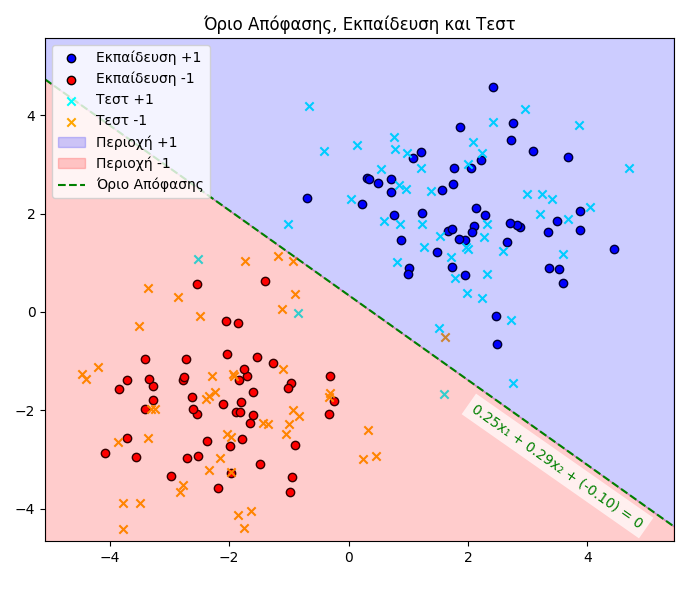
\includegraphics[height=6cm]{Samples.png}
        \caption{Απεικόνιση δεδομένων εκπαίδευσης, ελέγχου\\ και ορίου απόφασης}\label{fig:samples}
    \end{subfigure}
    \hfill
    \begin{subfigure}[t]{0.48\textwidth}
        \centering
        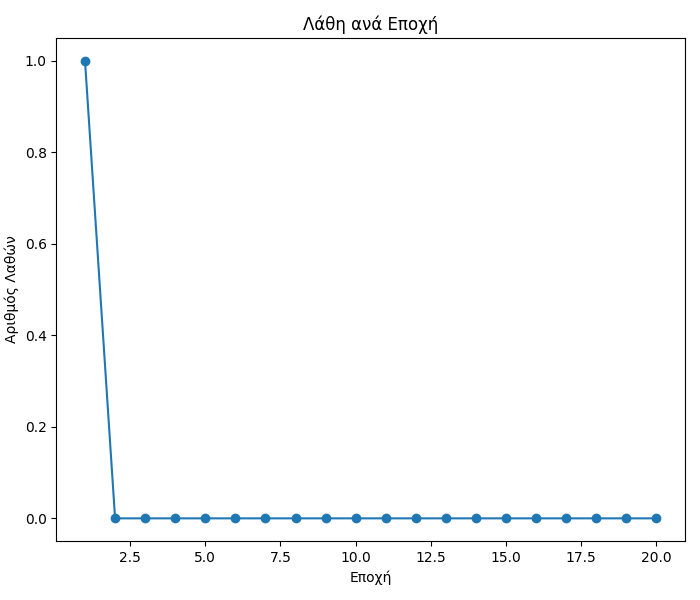
\includegraphics[height=6cm]{Errors.png}
        \caption{Γράφημα σφαλμάτων ανά εποχή εκπαίδευσης}\label{fig:errors}
    \end{subfigure}
    \caption{Οπτικοποίηση αποτελεσμάτων εκπαίδευσης του Perceptron}\label{fig:results}
\end{figure}

Στην Εικόνα~\ref{fig:results} παρουσιάζονται τα αποτελέσματα της εκπαίδευσης:
\begin{itemize}
    \item Εικόνα~\ref{fig:samples}: Σημεία εκπαίδευσης (μπλε/κόκκινο) και ελέγχου (κυανό/πορτοκαλί), καθώς και το όριο απόφασης (πράσινη διακεκομμένη γραμμή) που υπολόγισε το perceptron
    \item Εικόνα~\ref{fig:errors}: Ταχεία σύγκλιση του αλγορίθμου, με μόνο ένα σφάλμα στην πρώτη εποχή και μηδενικά σφάλματα στη συνέχεια
\end{itemize}

\printindex

% % Bibliography
% \bibliographystyle{plain}
% \bibliography{references}

% % Example citation
% ~\cite{example_reference}

\end{document} % chktex 17